\documentclass[10pt,a4paper,draft]{article}
\usepackage[utf8]{inputenc}
\usepackage{amsmath}
\usepackage{amsfonts}
\usepackage{amssymb}
\usepackage{relsize}
\usepackage{mathtools}
\usepackage[final]{graphicx}
\DeclareMathOperator*{\argmin}{argmin}
\newcommand*\perm[2][^n]{\prescript{#1\mkern-2.5mu}{}P_{#2}}
\begin{document}
\title{RL Formulation for the TSP Problem}
\author{Avrech Ben-David}
\maketitle


\section*{Problem Statement}
Given a graph $G(V,E)$, find the shortest tour path, such that every node in $V$ is visited only once. Representing the graph nodes as a list: $V = \{1,2,3,...,n\}$, the TSP solution $S$ is a permutation of $V$, such that:

\begin{equation} \label{tsp_statement}
	S = \argmin_{s \in P(V)} C(S)
\end{equation}

Where $C(S)$ is the TSP cost function - i.e. the tour path length:

\begin{equation}  \label{tsp_cost}
	C(S) := \mathlarger{\sum}_{i=1}^{|S|}{distance(s_i, s_{i+1})} + distance(s_{|S|}, s_i)
\end{equation}

Generally, the $distance(\cdot,\cdot)$ function can be any metric measure that fits the problem specifications.

Finding the optimal solution is a NP-hard problem. Exact solvers become slow on large problems. Furthermore, any change in the problem setting require visiting the exact algorithm again and adapt it to the modified problem.

TSP-solvers are often evaluated on the degenerated problem of fully-connected graphs, with the $2D euclidean$ metric. 

\section*{TSP RL Formulation}	
The TSP problem naturally lands to the RL standard formulation, mainly because the final $reward$ is well defined in the TSP problem statement itself. 
\cite{dai2017learning} use Q-Learning framework such that the tuple $\{S,A,R\}$ is defined as follows:
\begin{list}{}{}
	\item[•] State $S(k)$ - An ordered sequence of $k$ selected nodes $\in \perm[n]{k}$, representing the current partial solution.
	\item[•] Action $a(v)$ - Adding a node $v \not\in S(k)$ to the partial solution, and placing it greedily to minimize the increase in the $C(S)$. This comes with the transition from state $S$ to $S'$.
	\item[•] Reward $r(S,a)$ - The change in the cost function, after taking action $a$ in the state $S$ and transitioning to state $S'$, i.e. $C(S')-C(S)$
\end{list}

The cummulative $reward$ of the terminal state $\hat{S}$ concides exactly to the objective function, i.e. the total tour length:
Actually, we use the negative reward, so maximizing the reward is correlative minimizing the tour length.

\subsection*{Q-Learning}
We follow S2V paradigm of approximating the State-Action value function.
Designing the $Q(S,a)$ function is the main task of us. S2V-DQN uses a permutation invariant function, in the manner that it summes the partial solution nodes features. Probably it was designed at first for permutation-agnostic problems, such as MVC.

The desired $Q$ function has to be sensitive to the visiting order of the nodes, but must not overfit to specific input order. 

\cite{Bello} designed Pointer Network to learn a policy using policy gradient and actor-critic method. They also used MC estimator instead of TD(n). Pointer Network looks a natural choice to solve the TSP problem. The intuition behind using Monte Carlo for the TSP problem is that it captures the total tour length. TSP is not like common combinatorial problems (e.g. shortest path), where a partial solution is also the optimal solution for the corresponding reduced problem. So making greedy decisions might cost a lot at the end.
 
There are several works that follow \cite{Bello}, however, they do not show better performance. 
A partial list: \\

\cite{deudon-policy-gradient}, PN-AC-solver for ATSP\footnote{https://github.com/MichelDeudon/neural-combinatorial-optimization-rl-tensorflow}  \\

Decision version of TSP, use graph-embedding like S2V followed by PN-AC.





\section*{Experiments}
	The Concorde\footnote{https://github.com/jvkersch/pyconcorde} algorithm was used as the optimal solution, which the following approximation ratio and execution time ratio are related to. As a baseline model we took the cross-entropy method\footnote{https://github.com/v-iashin/CrossEntropyTSP}
\subsection*{Realworld Data - Experimental Setup}
	The results below refer to the Tsplib dataset\footnote{http://dimacs.rutgers.edu/Challenges/TSP/}. The dataset contains 38 cities of 51-318 nodes each one.
	The S2V model in this experiment was trained for 100,000 epochs on a single sample (berlin52). 
	Table \ref{tb_tsplib_performance_s2v_vs_ce} shows the averaged approximation and time ratio of S2V over the entire data-set. The ratio is defined as $\dfrac{S2V_{performance}}{Concorde_{performance}} $ so as the ratio is closer to 1 the S2V works better.
	
	\begin{table}[h] \centering
	\begin{tabular}{lll}
	 	Instance Name	& S2V   		& Cross-Entropy Method 	\\
	 	berlin52 		& 1.007@1.47	& - 					\\
		eil51  			& 1.049@1.73	& 1.16@5075				\\
		st70 			& 1.065@1.56 	& 1.17@16666 			\\
		eil76			& 1.066@3.45 	& 1.12@31000
	\end{tabular}
	\caption{Tsplib Small Cities Approximation Ratio vs Time} 
	\label{tb_tsplib_performance_s2v_vs_ce}
	\end{table}
	This experiment demonstrates the ability of S2V to solve an instance as an out-of-the-box solver\footnote{This was the answer I got for why did they trained the model on a single city only.}. 
	
	Additional experiments with traditional setting are detailed below. I did not evaluated the cross-entropy method on larger graphs than 80 nodes, because it becomes extremely slow. It takes around 11 minutes to solve a graph of 52 nodes, and it seems like it grows exponentially.
	

\subsection*{Synthetic Data Experiment}
In this experiment the network is trained on synthetic dataset\footnote{https://www.dropbox.com/sh/r39596h8e26nhsp/AADRm5mb82xn7h3BB4KXgETsa?dl=0}, consist of either clustered or uniformly distributed graphs.
I trained the network on 1000 graphs of 15-20 and 50-100 nodes. Table \ref{tb_tsp2d_performance_s2v} lists the achieved performance. 

\begin{table}[h] \centering
	\begin{tabular}{lll}
	 	Trained on		& Approximation @ Time Method 	\\
	 	15-20	 		& 1.092@0.91					\\
		50-100			& - 
	\end{tabular}
	\caption{Performance of S2V on TspLib for Different Train-set Size} 
	\label{tb_tsp2d_performance_s2v}
\end{table}

There is no significant improvement upon training on a single sample. It seems that this performance level really reflects the S2V architecture expressiveness.
	
\subsection*{The Paper Results}
	The table in Figure \ref{im_paper_aprx} shows the S2V approximation ratio as it was reported in the paper. The S2V approximation ratio on the TSP problem is approximately 1.1 for every train-test setup, in comparison to other problems (MVC, SCP etc.) where it shows outstanding perormance.
	\begin{figure}[h]
	\centering
	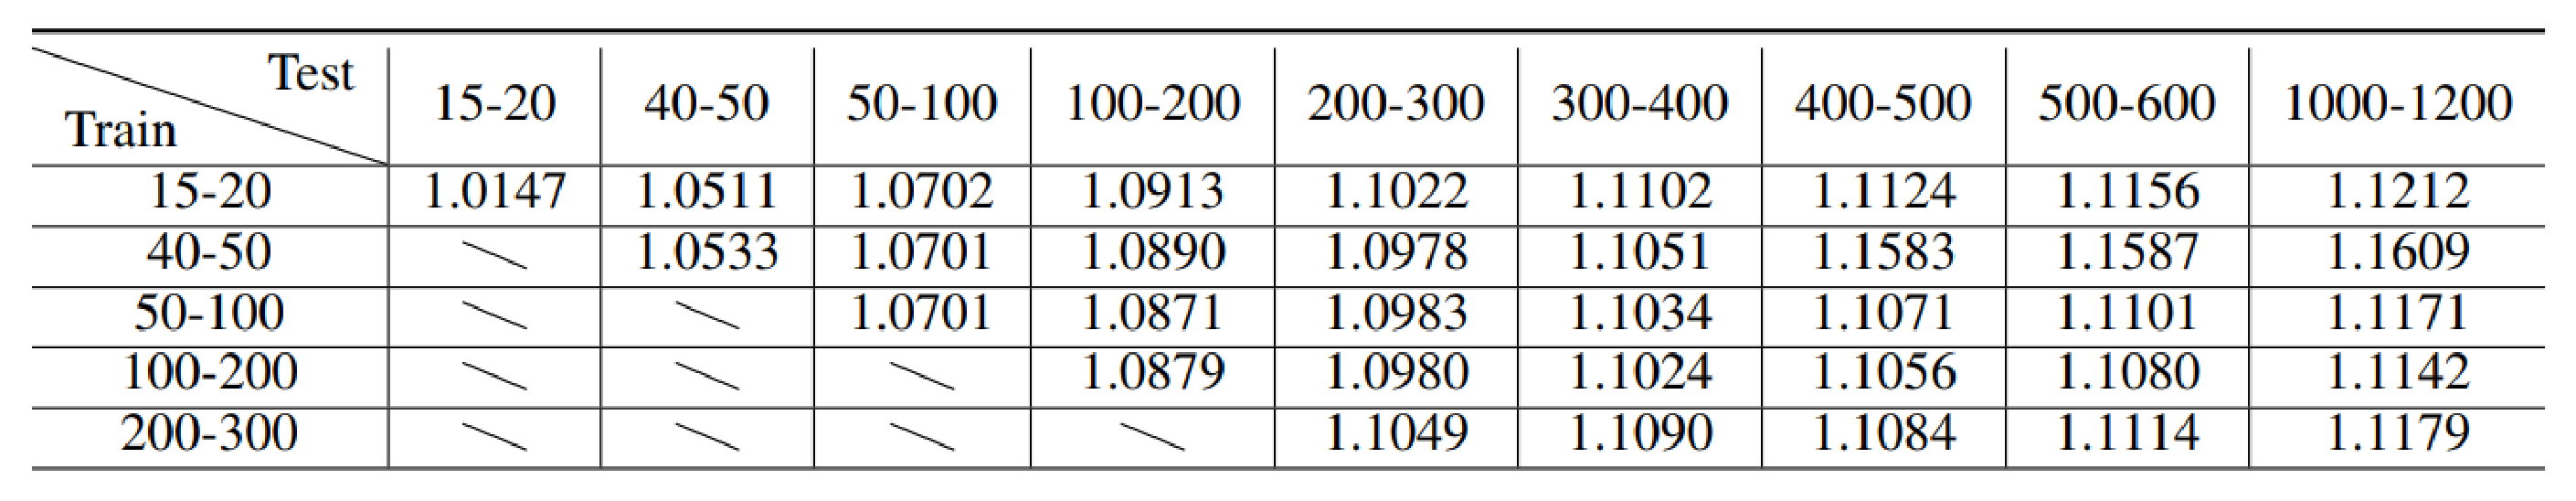
\includegraphics[width=1\textwidth]{tsp_paper_res_table.eps}
	\caption{Paper Approximation Ratio}
	\medskip
	\small
	Approximation ratio as function of the train-set and the test-set graphs' size. The efforts to train the network on larger graphs did not improve the performance significantly. For a certain test graph's size, the perfomance is roughly the same for all training sets. 
	\label{im_paper_aprx}
	\end{figure}
	
	\begin{figure}[h]
	\centering
	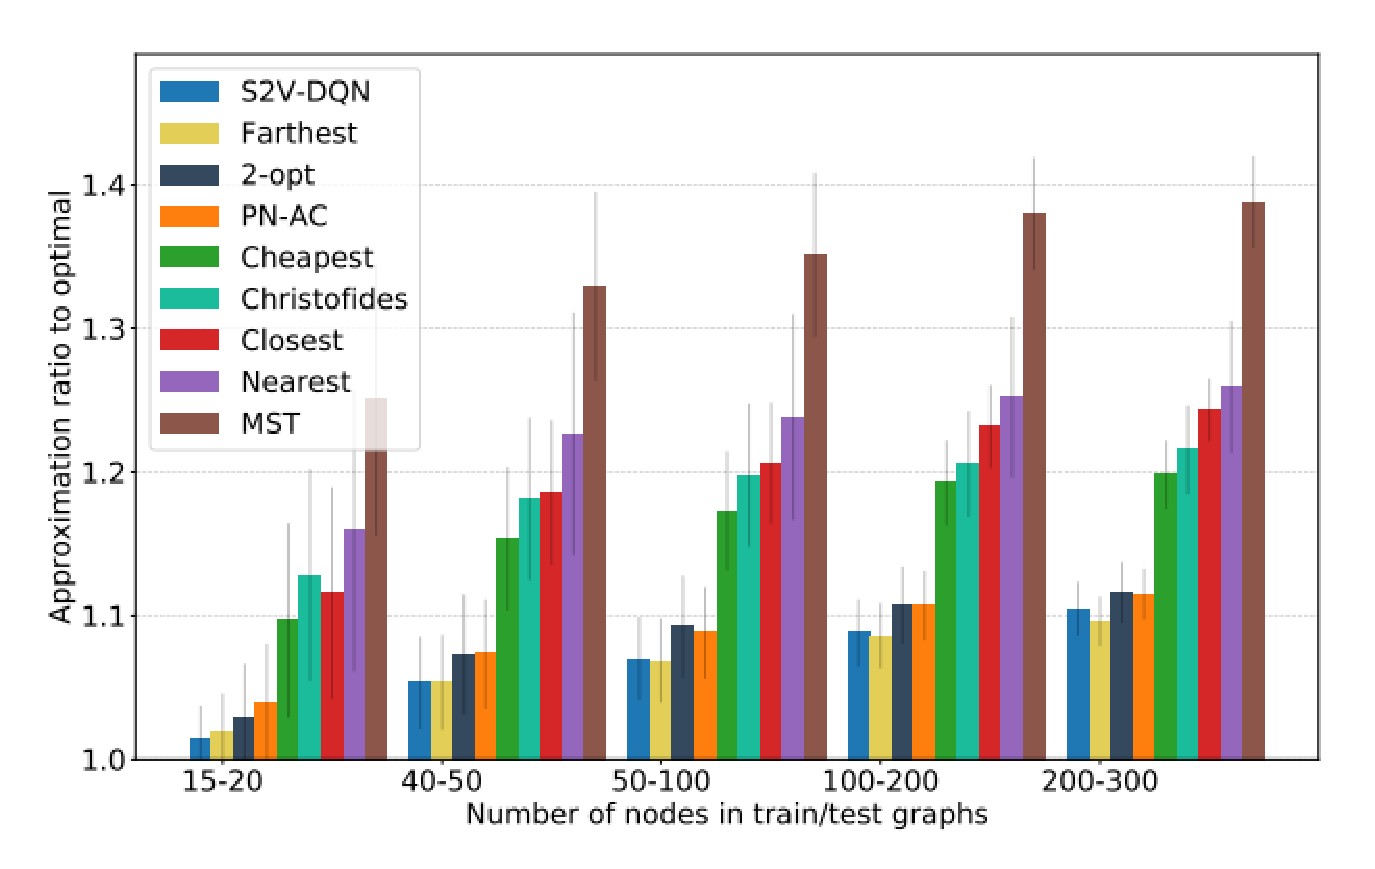
\includegraphics[width=1\textwidth]{tsp_paper_res_comp.eps}
	\caption{Approximation Ratio Comparison}
	\medskip
	\small
	A comparison of selected algorithms approximation ratio. S2V does not show outstanding performance, and even worse than other approximation methods.
	\label{im_paper_aprx_comp}
	\end{figure}
	 

\section*{The Authors Explanation}
	The authors explained the fact that S2V did not show impressive performance on the TSP problem in that the tested graphs are fully-connected. The graph structure is less important, and even "graph-agnostic" methods achieve the same performance. 
	Actually, the TSP problem was not widely investigated in the paper relative to the other problems.

\section*{My Conclusions}
	This work does not show outstanding performance on the TSP problem. The authors argue that it is because of the tested graphs are fully-connected, so that the 'graph structure' importance decreases, and the main advantage of the model doesn't expressed well. Such an argument should be supported in simple test. 
	
	I think that the S2V model has a built-in disadvantage regarding sequence mapping. The feedback that the model receivces from the currently constructed solution lacks the essential information about the tour path. The nodes features are summed together (in order to be invariant to permutations). It works well on MVC and probably on any other ${n \choose k}$-like problem, because the solution in such problems do not care of the nodes order. 
	In addition, some of the model's important properties are degenerated in this experiment, e.g. the n-step Q-learning. They do not give a satisfying intuition to their odd reward function (at least they say that it is a matter for future work).
	
	At the bottom-line, the S2V model, as is, do not fit the TSP problem's characteristics. 


\textbf{Experiment details as it is described in the paper}\footnote{https://arxiv.org/pdf/1704.01665.pdf}: \\

\bibliography{TSP_RL}
\bibliographystyle{plain}
\end{document}